\documentclass[class=article, crop=false]{standalone}
\usepackage{tikz}
\usepackage{subcaption}
\usetikzlibrary{calc}

\begin{document}
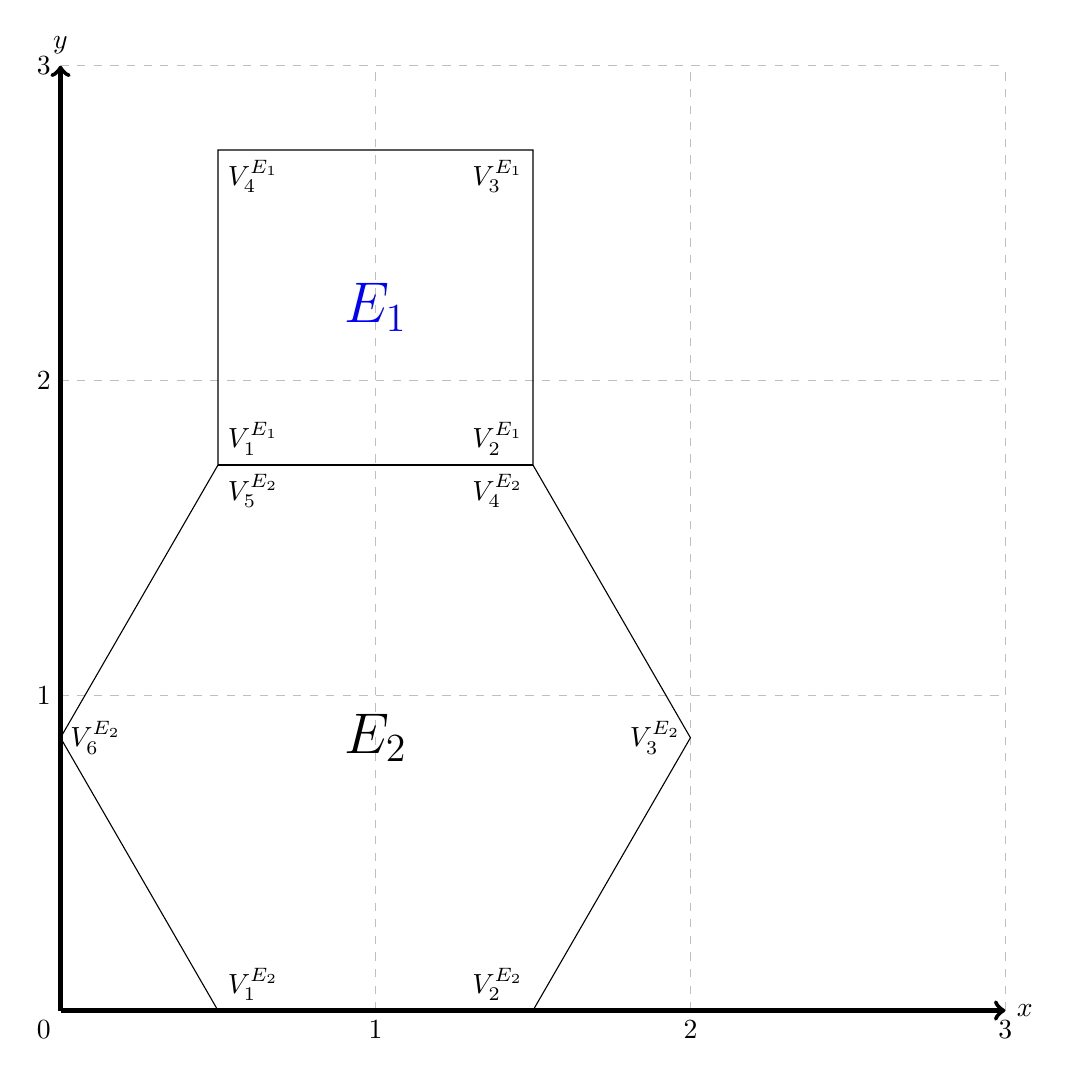
\begin{tikzpicture}[scale=4]
%Define Cooridinates
\coordinate (A) at (0.5,0);
\coordinate (B) at (1.5,0);
\coordinate (C) at (2,0.5*sqrt(3);
\coordinate (D) at (1.5,sqrt(3);
\coordinate (E) at (1.5,1+sqrt(3);
\coordinate (F) at (0.5,1+sqrt(3);
\coordinate (G) at (0.5,sqrt(3);
\coordinate (H) at (0, 0.5*sqrt(3);


%Axis
\draw[help lines, color=gray!50, dashed] (0,0) grid (3,3);
\draw[->,ultra thick] (0,0)--(3,0) node[right]{$x$};
\draw[->,ultra thick] (0,0)--(0,3) node[above]{$y$};

\draw (0,0) node [anchor = north east]{0};

\draw (0,1) node [anchor=east]{1};
\draw (0,2) node [anchor=east]{2};
\draw (0,3) node [anchor=east]{3};

\draw (1,0) node [anchor=north]{1};
\draw (2,0) node [anchor=north]{2};
\draw (3,0) node [anchor=north]{3};


%Lines and vertice labels.
\draw (A) node[anchor=south west]{$V^{E_2}_1$} 
-- (B) node[anchor=south east]{$V^{E_2}_2$} 
-- (C) node[anchor=east]{$V^{E_2}_3$} 
-- (D) node[anchor=north east]{$V^{E_2}_4$} 
-- (E) node[anchor=north east]{$V^{E_1}_3$} 
-- (F) node[anchor=north west]{$V^{E_1}_4$} 
-- (G) node[anchor=north west]{$V^{E_2}_5$} 
-- (H) node[anchor=west]{$V^{E_2}_6$} 
-- (A);
\draw (D) node[anchor=south east]{$V^{E_1}_2$}  
-- (G) node[anchor=south west]{$V^{E_1}_1$} ;

\node[black,rectangle] at (1,0.5*sqrt(3) {\huge $E_2$};
\node[blue,rectangle] at (1,0.5+sqrt(3) {\huge $E_1$};

\end{tikzpicture}
\end{document}